\section{8-Puzzle \cite{ai/book/Artificial-Intelligence-A-Modern-Approach/Russell-Norvig}}

\begin{table}[H]
\begin{minipage}[t]{0.45\linewidth}
\begin{figure}[H]
    \centering
    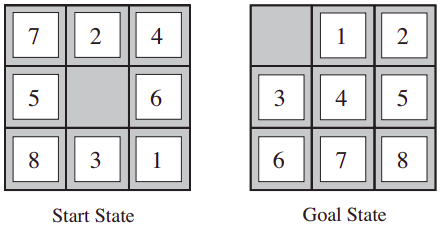
\includegraphics[
        width=\linewidth,
        height=4cm,
        keepaspectratio,
    ]{images/artificial-intelligence/examples/8-puzzle-instance-26steps.png}
    \caption{A typical instance of the 8-puzzle. The solution is 26 steps long.
    \cite{ai/book/Artificial-Intelligence-A-Modern-Approach/Russell-Norvig}}
    \label{fig:images/artificial-intelligence/examples/8-puzzle-instance-26steps.png}
\end{figure}
\end{minipage}
\hfill
\vrule
\hfill
\begin{minipage}[t]{0.45\linewidth}
\begin{figure}[H]
    \centering
    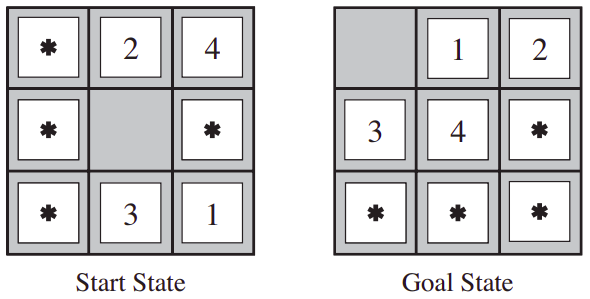
\includegraphics[
        width=\linewidth,
        height=4cm,
        keepaspectratio,
    ]{images/artificial-intelligence/examples/8-puzzle-instance-subprob-1234.png}
    \caption{A subproblem of the 8-puzzle instance.
    The task is to get tiles 1, 2, 3, and 4 into their correct positions, without worrying about what happens to the other tiles.
    \cite{ai/book/Artificial-Intelligence-A-Modern-Approach/Russell-Norvig}}
\end{figure}
\end{minipage}
\end{table}

\begin{enumerate}
    \item the objective of the puzzle is to slide the tiles horizontally or vertically into the empty space until the configuration matches the goal configuration
    \hfill \cite{ai/book/Artificial-Intelligence-A-Modern-Approach/Russell-Norvig}

    \item The average solution cost for a randomly generated 8-puzzle instance is about $22$ steps.
    The branching factor is about $3$.
    (When the empty tile is in the middle, four moves are possible; when it is in a corner, two; and when it is along an edge, three.)
    This means that an exhaustive tree search to depth $22$ would look at about $3^{22} \approx 3.1 \times 10^{10}$ states.
    A \textit{graph search} would cut this down by a factor of about $170,000$ because only $9!/2$ = $181, 440$ distinct states are reachable.
    \hfill \cite{ai/book/Artificial-Intelligence-A-Modern-Approach/Russell-Norvig}

    \item if the 8-puzzle actions are described as:
    \begin{enumerate}
        \item A tile can move from square A to square B \textbf{if} A is horizontally or vertically \textit{adjacent} to B \textbf{and} B is \textit{blank}
        \hfill \cite{ai/book/Artificial-Intelligence-A-Modern-Approach/Russell-Norvig}

        \item we can generate three relaxed problems by removing one or both of the conditions:
        \begin{enumerate}
            \item A tile can move from square A to square B if A is adjacent to B.
            \hfill \cite{ai/book/Artificial-Intelligence-A-Modern-Approach/Russell-Norvig}

            \item A tile can move from square A to square B if B is blank.
            \hfill \cite{ai/book/Artificial-Intelligence-A-Modern-Approach/Russell-Norvig}

            \item A tile can move from square A to square B.
            \hfill \cite{ai/book/Artificial-Intelligence-A-Modern-Approach/Russell-Norvig}
        \end{enumerate}
    \end{enumerate}
\end{enumerate}


\subsection{Comparing heuristic functions}

two commonly used candidates:
\begin{enumerate}
    \item $h_1$: the number of misplaced tiles.
    It is an \textbf{admissible} heuristic because it is clear that any tile that is out of place must be moved at least once.
    \hfill \cite{ai/book/Artificial-Intelligence-A-Modern-Approach/Russell-Norvig}
    \\
    All of the eight tiles are out of position, so the start state would have $h_1 = 8$.
    \hfill \cite{ai/book/Artificial-Intelligence-A-Modern-Approach/Russell-Norvig}

    \item $h_2$ = the sum of the distances of the tiles from their goal positions.
    (city block distance or Manhattan distance)
    h2 is \textbf{admissible} because all any move can do is move one tile one step closer to the goal.
    \hfill \cite{ai/book/Artificial-Intelligence-A-Modern-Approach/Russell-Norvig}
    \\
    $h_2 = 3 + 1 + 2 + 2 + 2 + 3 + 3 + 2 = 18$
    \hfill \cite{ai/book/Artificial-Intelligence-A-Modern-Approach/Russell-Norvig}
\end{enumerate}


\subsubsection{A$^\ast$ \cite{ai/book/Artificial-Intelligence-A-Modern-Approach/Russell-Norvig}}

\begin{enumerate}
    \item $N +1=1+ b^\ast + (b^\ast)^2 + \cdots + (b^\ast)^d$
    \hfill \cite{ai/book/Artificial-Intelligence-A-Modern-Approach/Russell-Norvig}

    \item if A$^\ast$ finds a solution at depth $5$ using $52$ nodes, then the effective branching factor is $1.92$
    \hfill \cite{ai/book/Artificial-Intelligence-A-Modern-Approach/Russell-Norvig}
\end{enumerate}



\subsubsection{Comparison \cite{ai/book/Artificial-Intelligence-A-Modern-Approach/Russell-Norvig}}

\begin{customArrayStretch}{1.3}
\begin{table}[h!]
\centering
\begin{tabular}{
|
>{\RaggedLeft\arraybackslash}p{1cm}||
>{\RaggedLeft\arraybackslash}p{1.7cm}|
>{\RaggedLeft\arraybackslash}p{1.7cm}|
>{\RaggedLeft\arraybackslash}p{1.7cm}||
>{\RaggedLeft\arraybackslash}p{1.7cm}|
>{\RaggedLeft\arraybackslash}p{1.7cm}|
>{\RaggedLeft\arraybackslash}p{1.7cm}|
}


\hline


\multirow{2}{*}{$d$} &
\multicolumn{3}{p{5.1cm}||}{\centering \textbf{Search Cost (nodes generated)}} &
\multicolumn{3}{p{5.1cm}|}{\centering \textbf{Effective Branching Factor}} \\

\cline{2-7}

&
IDS & A$^\ast$($h_1$) & A$^\ast$($h_2$) &
IDS & A$^\ast$($h_1$) & A$^\ast$($h_2$) \\

\hline \hline


$2$  & $10$      & $6$     & $6$     & $2.45$ & $1.79$ & $1.79$ \\ \hline
$4$  & $112$     & $13$    & $12$    & $2.87$ & $1.48$ & $1.45$ \\ \hline
$6$  & $680$     & $20$    & $18$    & $2.73$ & $1.34$ & $1.30$ \\ \hline
$8$  & $6384$    & $39$    & $25$    & $2.80$ & $1.33$ & $1.24$ \\ \hline
$10$ & $47127$   & $93$    & $39$    & $2.79$ & $1.38$ & $1.22$ \\ \hline
$12$ & $3644035$ & $227$   & $73$    & $2.78$ & $1.42$ & $1.24$ \\ \hline
$14$ & $-$       & $539$   & $113$   & $-$    & $1.44$ & $1.23$ \\ \hline
$16$ & $-$       & $1301$  & $211$   & $-$    & $1.45$ & $1.25$ \\ \hline
$18$ & $-$       & $3056$  & $363$   & $-$    & $1.46$ & $1.26$ \\ \hline
$20$ & $-$       & $7276$  & $676$   & $-$    & $1.47$ & $1.27$ \\ \hline
$22$ & $-$       & $18094$ & $1219$  & $-$    & $1.48$ & $1.28$ \\ \hline
$24$ & $-$       & $39135$ & $1641$  & $-$    & $1.48$ & $1.26$ \\ \hline


\end{tabular}
\caption{
Comparison of the search costs and effective branching factors for the \textsc{Iterative-Deepening-Search} and A$^\ast$ algorithms with $h_1$, $h_2$.
\\
Data are averaged over $100$ instances of the $8$-puzzle for each of various solution lengths $d$.
\cite{ai/book/Artificial-Intelligence-A-Modern-Approach/Russell-Norvig}
}
\end{table}
\end{customArrayStretch}


\begin{enumerate}
    \item $h_2$ is always better than $h_1$.
    for any node $n$, $h_2(n) \geq h_1(n)$.
    \hfill \cite{ai/book/Artificial-Intelligence-A-Modern-Approach/Russell-Norvig}

    \item $h_1$ and $h_2$ are \textbf{estimates} of the remaining path length for the $8$-puzzle, but they are also \textbf{perfectly accurate} path lengths for \textbf{simplified versions} of the puzzle.
    \hfill \cite{ai/book/Artificial-Intelligence-A-Modern-Approach/Russell-Norvig}


\end{enumerate}




\subsubsection{Generating admissible heuristics from subproblems: Pattern databases}

\begin{enumerate}
    \item[] \textbf{Relaxed Sub-problem method}

    \item The choice of 1-2-3-4 is fairly arbitrary; we could also construct databases for 5-6-7-8, for 2-4-6-8, and so on.
    \hfill \cite{ai/book/Artificial-Intelligence-A-Modern-Approach/Russell-Norvig}

    \item the heuristics obtained from the 1-2-3-4 database and the 5-6-7-8 \textbf{cannot} be added
     because the solutions of the 1-2-3-4 subproblem and the 5-6-7-8 subproblem for a given state will almost certainly share some moves—it is unlikely that 1-2-3-4 can be moved into place without touching 5-6-7-8, and vice versa.
    \hfill \cite{ai/book/Artificial-Intelligence-A-Modern-Approach/Russell-Norvig}

    \item[] \textbf{Experience method}

    \item “Experience” here means solving lots of $8$-puzzles.
    Each optimal solution to an 8-puzzle problem provides examples from which $h(n)$ can be learned.
    Each example consists of a state from the solution path and the actual cost of the solution from that point.
    \hfill \cite{ai/book/Artificial-Intelligence-A-Modern-Approach/Russell-Norvig}

    \item From these examples, a learning algorithm can be used to construct a function $h(n)$ that can (with luck) predict solution costs for other states that arise during search.
    Techniques for doing this use neural nets, decision trees, and other methods or reinforcement learning.
    \hfill \cite{ai/book/Artificial-Intelligence-A-Modern-Approach/Russell-Norvig}
\end{enumerate}
















